\documentclass[11pt,a4paper]{article}
\usepackage[utf8]{inputenc}
\usepackage[spanish]{babel}
\usepackage{amsmath}
\usepackage{amsfonts}
\usepackage{amssymb}
\usepackage[export]{adjustbox}
\usepackage{tabularx}
\usepackage[table]{xcolor}
\usepackage{float}
\usepackage{url}
\usepackage{hyperref}
\hypersetup{
    colorlinks=true,
    linkcolor=black,
    filecolor=black,      
    urlcolor=blue,
    citecolor=blue,
}
\usepackage{graphicx}
\graphicspath{ {images/} }


\begin{document}


\begin{titlepage}

\includegraphics[scale=0.2,right,valign=t]{uoc-logo.png}
\vspace*{\fill}
\begin{flushleft}
{\LARGE \textbf{YouTubeCrawlerTool: Aplicación web para habilitar el estudio del movimiento antivacuna en YouTube}}
\end{flushleft}
\begin{flushleft}
\textbf{Javier Sánchez Mendoza}\\
Grado de ingeniería informática\\
Health IT
\end{flushleft}
\begin{flushleft}
\textbf{Carlos Luis Sánchez Bocanegra}\\
\textbf{José Antonio Morán Moreno}
\end{flushleft}
\begin{flushleft}
Junio de 2018  
\end{flushleft}
\end{titlepage}


\begin{titlepage}
\vspace*{\fill}
\begin{flushleft}

\includegraphics[scale=1,left]{licencia-cc.png}
Esta obra está sujeta a una licencia de\\
Reconocimiento-NoComercial-SinObraDerivada\\
\href{http://creativecommons.org/licenses/by-nc-nd/3.0/es/}{3.0 España de Creative Commons}
\end{flushleft}
\end{titlepage}



\begin{flushleft}
\textit{Quiero dedicar este trabajo especialmente a:}
\linebreak
 
\textbf{\textit{Carolina}} \\
\textit{Por empujarme a retomar mis estudios y, lo que es mas importante, motivarme durante todo este tiempo.}
\linebreak

\textbf{\textit{Amy, Luke y Jim}}\\
\textit{Por obligarme a salir a la calle de vez en cuando y estar siempre hay.}
\linebreak
\end{flushleft}
\newpage 



\begin{center}
\textbf{FICHA DEL TRABAJO FINAL}
\end{center}
\begin{tabularx}{\textwidth}{|X|X|}
\hline 
\textbf{Título del trabajo:} &\cellcolor{gray!25} \textit{YouTubeCrawlerTool: Aplicación web para habilitar el estudio del movimiento antivacuna en YouTube} \\ 
\hline 
\textbf{Nombre del autor:} &\cellcolor{gray!25} \textit{Javier Sánchez Mendoza} \\ 
\hline 
\textbf{Nombre del consultor/a:} &\cellcolor{gray!25} \textit{Carlos Luis Sánchez Bocanegra} \\ 
\hline 
\textbf{Nombre del PRA:} &\cellcolor{gray!25} \textit{José Antonio Morán Moreno} \\ 
\hline 
\textbf{Fecha de entrega:} &\cellcolor{gray!25} \textit{06/2018} \\ 
\hline 
\textbf{Titulación:} &\cellcolor{gray!25} \textit{Grado de ingeniería informática} \\ 
\hline 
\textbf{Área del Trabajo Final:} &\cellcolor{gray!25} \textit{Health IT} \\ 
\hline 
\textbf{Idioma del trabajo:} &\cellcolor{gray!25} \textit{Español} \\ 
\hline 
\textbf{Palabras clave:} &\cellcolor{gray!25} \textit{antivacuna, crawler, YouTube.} \\ 
\hline
\end{tabularx} 
\begin{tabularx}{\textwidth}{|X|}
\textbf{Resumen del Trabajo (máximo 250 palabras):} \textit{Con la finalidad, contexto de aplicación, metodología, resultados i conclusiones del trabajo.} \\ 
\hline 
\cellcolor{gray!25} \textit{...} \\
\hline 
\end{tabularx} 
\newpage 


\begin{tabularx}{\textwidth}{|X|}
\hline 
\textbf{Abstract (in English, 250 words or less):} \\ 
\hline 
\cellcolor{gray!25} \textit{...} \\
\hline 
\end{tabularx} 
\newpage 


\tableofcontents
\newpage


\listoffigures
\newpage


\section{Introducción}
\bigskip 

\subsection{Contexto y justificación del Trabajo}
Desde la introducción de la vacunación como método preventivo de enfermedades han existido entidades y grupos de personas que se han opuesto a ella y han dudado de su efectividad o propósito \cite{1}. Hoy en día el activismo anti-vacunación (conocido también como movimiento antivacunas) ha vuelto a la actualidad y se encuentra en auge en algunas regiones tales como Europa o Estados Unidos, cobrándose en el peor de los escenarios victimas mortales a causa de enfermedades que se creían erradicadas y que han vuelto a surgir \cite{2}\cite{3}.
\\

Para hacer posible el estudio y comprensión de las motivaciones del movimiento antivacuna y luchar contra su desinformación, se propone el desarrollo de una aplicación que permita la recolección de grandes cantidades de datos de la actividad realizada por parte de este colectivo en redes sociales con el fin de hacer posible su posterior tratamiento y estudio para obtener valor añadido. Para tal fin, en este proyecto contamos con la colaboración de Johanna Milena Rodríguez Vera estudiante de master en Telemedicina que asume el rol de analista de datos (\textit{data scientist} \cite{4}) en el desarrollo de su trabajo final de máster titulado \textit{Evaluación de la información sanitaria en vacunas disponible en las redes sociales - YouTube} y que actúa a la vez como clienta de la aplicación desarrollada en el presente proyecto.
\\

Hoy en día las redes sociales han puesto al alcance de los analistas de datos una gran cantidad de información disponible para ser analizada, una de las problemáticas a las que se quiere hacer frente es la obtención de dichos datos de forma efectiva. Para ello se propone hacer uso de interfaces de programación de aplicaciones (abreviado como \textit{API} \cite{5} en ingles) ofrecidas públicamente por distintas redes sociales de tal forma que el proceso resulte transparente para el usuario final, permitiéndole la extracción a este problema.
\\

La obtención de grandes volúmenes de datos nos lleva también a la problemática que surge en su almacenamiento en bases de datos tradicionales y su posterior procesamiento. Para habilitar al usuario final el correcto acceso a la información obtenida se estudían las ventajas que aporta el uso de bases de datos \textit{NoSQL} \cite{6} para este cometido, al ser diseñadas especialmente para manejar enormes cantidades de datos. Proyecto que se enmarca dentro de la problemática de la obtención, almacenamiento y procesamiento de grandes volúmenes de datos (\textit{Big Data} \cite{7}) y su posterior acceso.
\newpage

\subsection{Objetivos del Trabajo}
El objetivo principal del proyecto es proporcionar una aplicación web que permita a la clienta obtener de forma usable y transparente la información que necesite de la red social \textit{YouTube} para poder llevar a cabo el estudio de patrones de comportamiento entre las diferentes movimientos anti y pro vacuna.
\\

Entre los objetivos secundarios del proyecto se encuentra la exploración de otras redes sociales y proporcionar una herramienta lo suficientemente genérica para que pueda ser utilizada en la investigación realizada por Johanna así como en otras investigaciones futuras de distinta temática.
\\

Algunos objetivos concretos que se han querido lograr son los siguientes: 
\begin{itemize}
\item Investigar que funcionalidades aportan las \textit{API} públicas ofrecidas por \textit{YouTube} y analizar como se pueden utilizar para la obtención de la información requerida.
\item Determinar como almacenar y acceder de forma eficiente a la gran cantidad de información que se obtendrá.
\item Permitir la recolección de información según criterios de búsqueda proporcionados por el usuario final.
\item Habilitar la gestión, visualización y exportación de datos obtenidos en distintos procesos de extracción para su posterior análisis en herramientas especializadas.
\item Ofrecer herramientas de visualización para el análisis y comprensión de los datos obtenidos.
\item Proporcionar una interfaz de usuario usable que permita realizar las acciones requeridas por el usuario final.
\end{itemize}
\medskip 

\subsection{Enfoque y método seguido}
Para la realización del proyecto se ha seguido el marco ágil de desarrollo \textit{scrum} \cite{8}. Al adoptar esta metodología como marco de trabajo nos ha permitido, a diferencia de otras metodologías lineales de desarrollo como pueden ser los modelos en cascada, poder desarrollar el proyecto de forma flexible permitiéndonos adaptar la planificación inicial del proyecto en los casos necesarios para adecuarse a los nuevos requerimientos.
\\

La forma en la cual se aplico la metodología \textit{scrum} en el proyecto esta condicionada por los integrantes del equipo de desarrollo, en el cual la figura del \textit{product owner}, \textit{scrum master} y desarrollador recaen sobre la figura del alumno que presenta el actual proyecto descrito (Javier Sánchez Mendoza), mientras que la figura del cliente estará representada por una analista de datos (Johanna Milena Rodríguez Vera) y el consultor de los mismos (Carlos Luis Sánchez Bocanegra) como \textit{stakeholder}.
\\

Siguiendo la metodología \textit{scrum}, se realizaron iteraciones (comúnmente conocidos como \textit{sprints}) de una semana de duración donde, en la finalización de los mismos, se realizaron reuniones online para revisar y aprobar las tareas realizadas (\textit{sprint review}) y definir las tareas para la siguiente iteración (\textit{sprint planning}). Para gestionar las tareas a realizar (\textit{backlog}) se decidio utilizar la herramienta online \textit{Trello} \cite{9}:
\\

\begin{figure}[hbtp]
\centering
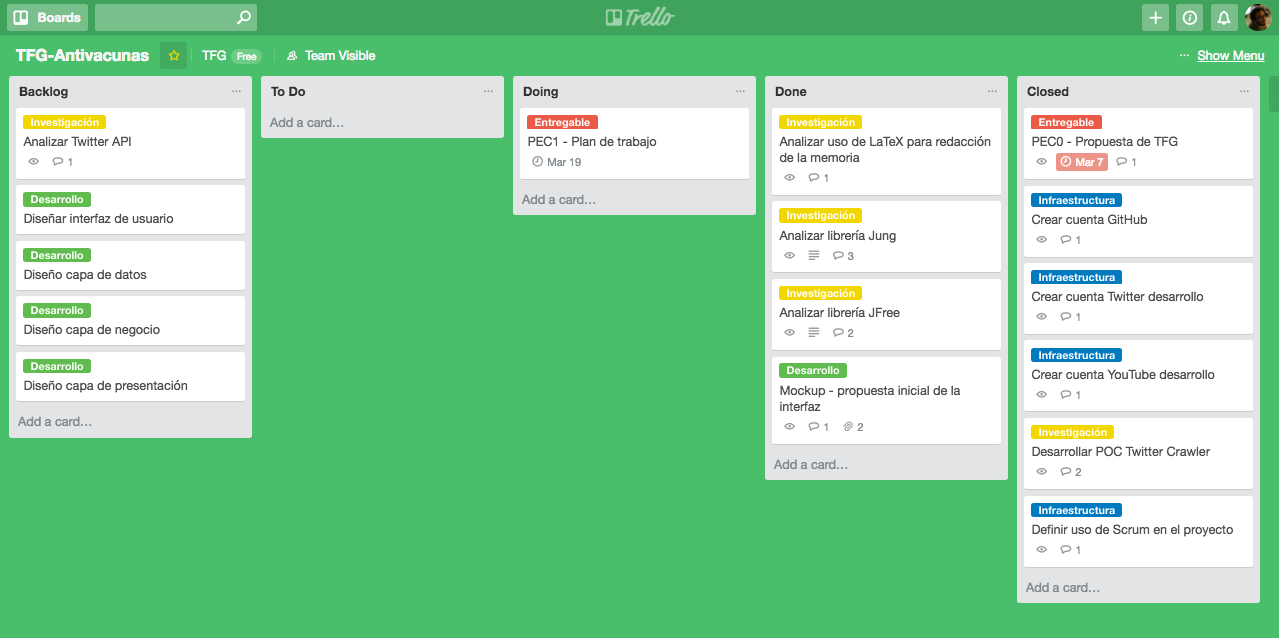
\includegraphics[scale=0.3]{planificacion/trello-backlog.png}
\caption{Ejemplo del backlog del proyecto en Trello}
\end{figure}
\medskip 

\subsection{Planificación del Trabajo}
En la realización del proyecto se propuso inicialmente seguir una planificación tentativa tal y como se detalla en el diagrama de \textit{Grantt} facilitado en las figuras dos y tres:

\begin{figure}[H]
\centering
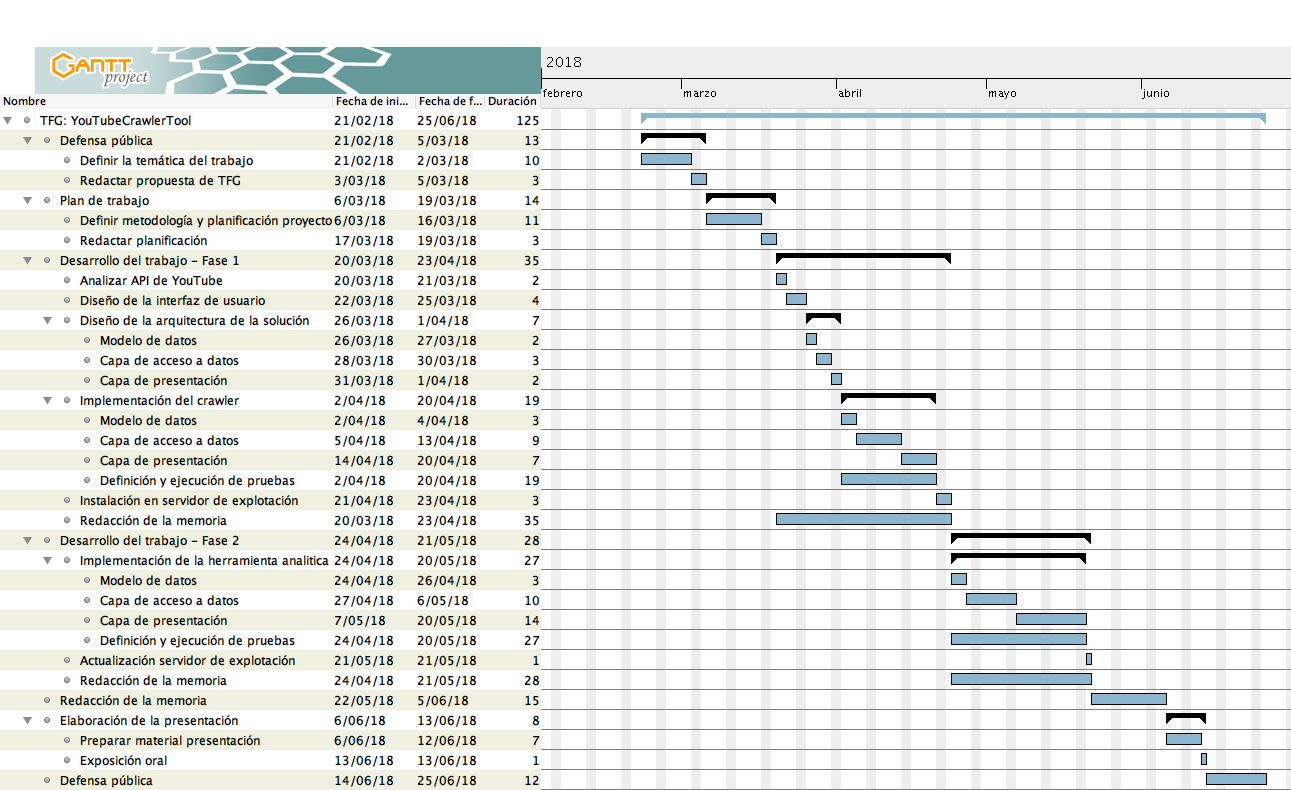
\includegraphics[scale=0.25]{planificacion/planificacion.png}
\caption{Listado de tareas y diagrama de Gantt}
\end{figure}

\begin{figure}[H]
\centering
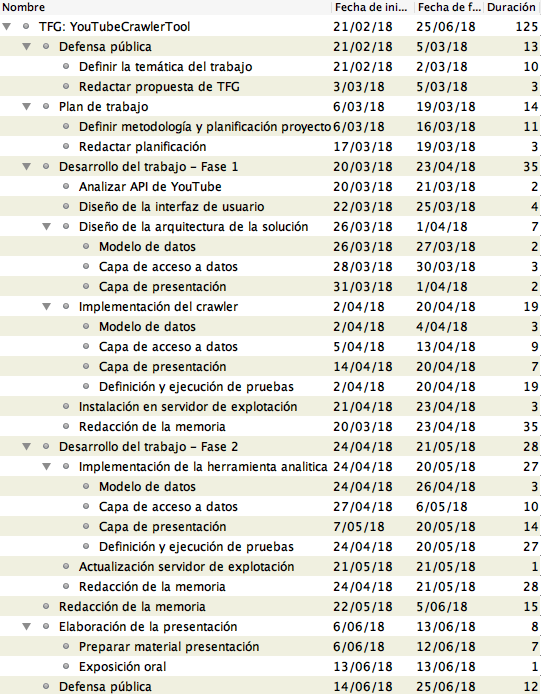
\includegraphics[scale=0.4]{planificacion/listado-tareas.png}
\caption{Listado de tareas}
\end{figure}
\newpage

De la planificación inicial cabe destacar que la redacción de la memoria se diseño como una tarea evolutiva que se desarrollaría durante todas las fases del proyecto pero mas intensamente durante la antepenúltima fase dedicada exclusivamente a su redacción. Además, durante las dos fases de desarrollo se  planificaron dos tareas recurrentes para la definición y realización de pruebas de calidad del producto a realizar durante todo el ciclo de desarrollo.
\\

Como se puede observar, en el diagrama facilitado en cada entrega se pretendían conseguir unos hitos concretos. La relación de los mas destacables por entrega son los siguientes:

\begin{itemize}
\item \textbf{Definición de los contenidos del trabajo:} Redacción propuesta TFG.
\item \textbf{Plan de trabajo:} Redacción planificación.
\item \textbf{Desarrollo del trabajo – Fase 1:} Instalación en servidor de explotación de la primera versión de la aplicación con funcionalidad de \textit{crawler} implementada.
\item \textbf{Desarrollo del trabajo – Fase 2:} Actualización en servidor de explotación de la versión final de la aplicación con funcionalidad analítica implementada.
\item \textbf{Redacción de la memoria:} Entrega de la memoria del proyecto.
\item \textbf{Elaboración de la presentación:} Realizar exposición oral.
\item \textbf{Defensa pública:} Defender públicamente el proyecto.
\end{itemize}

Los riesgos detectados en la planificación inicial se concentraban principalmente en la consecución del hito definido en la primera fase de desarrollo. Para permitir a la clienta de la aplicación poder empezar a recopilar datos para su investigación lo antes posible, se decidió realizar la instalación de la aplicación desarrollada en un entorno de explotación en dos fases distintas, una con la funcionalidad del \textit{crawler} y otra con la funcionalidad analítica implementada. La demora en la primera fase de desarrollo podría comprometer el éxito de la investigación del cliente. Para mitigar este riesgo se realizo el seguimiento del mismo durante las diferentes iteraciones en esa fase de desarrollo. 
\\

Cabe destacar que el diagrama proporcionado en esta sección representa la estimación inicial de la planificación del proyecto de forma tentativa y fue sujeto a modificaciones al inicio de cada nueva fase de desarrollo para garantizar el éxito del proyecto. En la sección de conclusiones del presente documento en el apartado \ref{sec:seguiminetoPlanificacion} se realiza una comparación entre la planificación inicial y sus respectivas revisiones.
\newpage


\subsection{Arquitectura tecnológica}
Para la consecución de los objetivos definidos se ha desarrollado una aplicación web bautizada como \textit{YouTubeCrawlerTool} la cual ha sido diseñada por capas.
\\

La capa de negocio de dicha aplicación ha sido desarrollada con tecnología Java EE \cite{10} implementada mayormente utilizando proyectos del marco de desarrollo Spring Framework \cite{11} entre otros. En esta capa se hace uso intensivo de servicios externos en forma de API pública ofrecida por YouTube con el fin de consumir dicha API para recolectar los vídeos requeridos por el usuario para su estudio.
\\

En la capa de presentación se ha utilizado el lenguaje JavaScript \cite{12} con un gran uso de JQuery \cite{13} para modificar el DOM de las vistas y realizar llamadas asíncronas a la API Rest habilitada en la capa de negocio para tales efectos.
\\

Finalmente, en la capa de datos se utiliza una base de datos orientada a grafos \cite{14} la cual nos permite persistir los vídeos obtenidos en forma de grafo junto con sus relaciones ademas de otras informaciones derivadas y necesarias para el uso y funcionamiento de la aplicación.
\\

En los siguientes apartados se profundiza en la arquitectura y el diseño de la aplicación introducidos en esta sección.
\medskip 

\subsection{Resumen de capítulos}
En los próximos capítulos se detalla el trabajo realizado juntamente con los productos obtenidos y sus conclusiones. La relación de capítulos es la siguiente:

\begin{itemize}
\item \textbf{Análisis y diseño:} Explicación de la metodología de diseño escogida así como los pasos que se llevaron a cabo para definir una propuesta a la clienta y su posterior análisis para acabar definiendo la arquitectura de la solución.
\item \textbf{Desarrollo:} Descripción del desarrollo efectuado y de las decisiones realizadas durante el proceso.
\item \textbf{Implementación y puesta en funcionamiento:} Detalle de los productos obtenidos con las instrucciones para su correcta puesta en funcionamiento ademas de las acciones de formación realizadas.
\item \textbf{Conclusiones:} Sumario de resultados obtenidos y conclusiones sobre el trabajo realizado.
\end{itemize}

\newpage 



\section{Análisis y diseño}
\bigskip 

\subsection{Metodología}\label{metodologia} 
Para realizar el diseño de la aplicación se opto de entre diferentes posibilidades el enfoque definido por la filosofía del 'Diseño centrado en el usuario' \cite{15}.
\\

El diseño centrado en el usuario, como bien indica su nombre, se caracteriza por conocer a fondo a los futuros usuarios de una aplicación para diseñar un producto que resuelva sus necesidades y expectativas buscando en todo momento conseguir la mayor satisfacción del usuario posible. Se trata de un proceso iterativo y cíclico por fases en donde en cada una de ellas se utilizan distintas técnicas para conseguir los objetivos propuestos. 
\\

En nuestro proyecto se ha decidido seguir esta y no otra metodología de diseño tales como el 'Diseño centrado en la actividad' o el 'Diseño centrado en el uso' debido a que, como en nuestro caso la clienta de la aplicación va a ser también la usuaria final de la misma, se ha decidido realizar el análisis de la aplicación centrada en ella y sus necesidades por encima de la actividad que se llevara a cabo o el uso.
\\

La relación de fases y técnicas utilizadas ha sido la siguiente:

\begin{itemize}
\item \textbf{Definir contexto de uso:} El objetivo de esta fase es el de determinar que necesidades pretende la usuaria final que la aplicación resuelva y a que se va a destinar su uso. La técnica escogida para la realización de esta fase fueron las entrevistas con la usuaria final que se realizaron mediante videoconferencia sobretodo durante las diferentes \textit{sprint reviews} al termino de cada \textit{sprint}.
\item \textbf{Especificar requisitos:} En la siguiente fase se definen los requisitos del sistema a partir de la información recogida en la fase previa. Para los requisitos funcionales se opto por recogerlos como 'casos de uso' \cite{16}.
\item \textbf{Diseñar el producto:} En esta fase se diseñan y implementan los requisitos definidos en la fase anterior ya sea con el objetivo de proporcionar una solución final o una propuesta de solución a ser refinada en sucesivas iteraciones. Las técnicas utilizadas en esta fase fueron la creación de maquetas para evaluar la solución y el prototipado mediante pruebas de concepto realizadas con el objetivo de estudiar posibles soluciones antes de realizar su implementación en la aplicación.
\item \textbf{Poner a prueba el producto:} Finalmente, en esta fase se pone a prueba el producto obtenido. Para hacerlo, se definieron y ejecutaron pruebas de integración diseñadas teniendo en cuenta los casos de uso definidos previamente y se realizaron test con usuarios para evaluar su grado de satisfacción.
\end{itemize}

Gracias al enfoque escogido fue posible encontrar respuestas a preguntas sobre las expectativas que la usuaria tenia depositadas sobre la aplicación y que fueron de gran ayuda a la hora de diseñar la solución final. Algunas de las principales preguntas fueron:\\
\textit{¿Quiénes son los usuarios de la aplicación?}\\
\textit{¿Cuáles son las tareas a realizar?}\\
\textit{¿Qué funcionalidades se necesitan?}\\
\textit{¿Qué información se necesita?}
\\

También cabe destacar que gracias a que tanto \textit{scrum} como el diseño centrado en el usuario son dos procesos iterativos, resulto fácil integrar esta metodología dentro del marco ágil de desarrollo.
\medskip 

\subsection{Propuesta de la solución}
\medskip 

\subsubsection{Reuniones y entrevistas}
Tal y como se ha introducido en la sección \ref{metodologia} sobre la metodología de diseño utilizada, para definir el contexto de uso y conocer las necesidades a ser cubiertas por la aplicación, se realizaron varias entrevistas con la clienta y los \textit{stakeholders} donde la gran mayoría de ellas fueron dentro del contexto de \textit{scrum} como reuniones de \textit{sprint review} y \textit{sprint planning}.
\\

A continuación se resumen las entrevistas y reuniones realizadas junto con los principales temas tratados y decisiones tomadas:
\\

\noindent\textbf{Fecha:} 05/03/2018
\\
\noindent\textbf{Hora de inicio:} 21:00
\\
\noindent\textbf{Hora final:} 21:45
\\
\noindent\textbf{Asistentes:} 
\begin{itemize}
\item Carlos Luis Sánchez Bocanegra: \textit{stakeholder}
\item Johanna Milena Rodríguez Vera: clienta
\item Javier Sánchez Mendoza: \textit{product owner}, \textit{scrum master} y desarrollador
\end{itemize}
\noindent\textbf{Temas tratados:}
\begin{itemize}
\item Que conocimiento sobre el movimiento antivacunas se quiere obtener. 
\item Que se pretende hacer con la información recolectada.
\item Definición de los objetivos de la aplicación.
\end{itemize}
\noindent\textbf{Decisiones:}
\begin{itemize}
\item La clienta definirá los criterios de búsqueda y el conocimiento que debe ser obtenido por la aplicación.
\item El análisis de los datos los realizara la clienta con herramientas especializadas.
\item El objetivo principal de la aplicación es la obtención de datos mediante búsquedas en redes sociales.
\item La aplicación debe ofrecer funcionalidad para exportar los datos recolectados a otras herramientas.
\end{itemize}

\begin{center}\rule{10cm}{0.4pt}\end{center}

\noindent\textbf{Fecha:} 12/03/2018
\\
\noindent\textbf{Hora de inicio:} 21:00
\\
\noindent\textbf{Hora final:} 21:30
\\
\noindent\textbf{Asistentes:} 
\begin{itemize}
\item Carlos Luis Sánchez Bocanegra: \textit{stakeholder}
\item Johanna Milena Rodríguez Vera: clienta
\item Javier Sánchez Mendoza: \textit{product owner}, \textit{scrum master} y desarrollador
\end{itemize}
\noindent\textbf{Temas tratados:}
\begin{itemize}
\item Alcance del estudio a realizar.
\item Sobre que redes sociales debe centrarse el estudio.
\end{itemize}
\noindent\textbf{Decisiones:}
\begin{itemize}
\item Se decide adoptar el marco de trabajo \textit{scrum} para la realización del proyecto.
\item El \textit{product owner} realizara una propuesta inicial de la interfaz de usuario.
\end{itemize}

\begin{center}\rule{10cm}{0.4pt}\end{center}

\noindent\textbf{Fecha:} 19/03/2018
\\
\noindent\textbf{Hora de inicio:} 21:00
\\
\noindent\textbf{Hora final:} 21:30
\\
\noindent\textbf{Asistentes:} 
\begin{itemize}
\item Carlos Luis Sánchez Bocanegra: \textit{stakeholder}
\item Johanna Milena Rodríguez Vera: clienta
\end{itemize}
\noindent\textbf{Temas tratados:}
\begin{itemize}
\item Comentarios sobre la propuesta inicial de la interfaz de usuario realizada por el \textit{product owner}.
\item Pros y contras sobre la elección de \textit{Twitter} como red social para el estudio.
\end{itemize}
\noindent\textbf{Decisiones:}
\begin{itemize}
\item Elección de \textit{Twitter} como red social a utilizar en el estudio.
\item La aplicación incluirá una visualización en forma de grafo para poder estudiar la relación existente entre la información recolectada.
\item Seguir refinando la propuesta de interfaz de usuario.
\item El \textit{product owner} debe estudiar la viabilidad de utilizar \textit{Twitter} para la consecución de los objetivos. 
\end{itemize}

\begin{center}\rule{10cm}{0.4pt}\end{center}

\noindent\textbf{Fecha:} 26/03/2018
\\
\noindent\textbf{Hora de inicio:} 21:00
\\
\noindent\textbf{Hora final:} 21:45
\\
\noindent\textbf{Asistentes:} 
\begin{itemize}
\item Carlos Luis Sánchez Bocanegra: \textit{stakeholder}
\item Johanna Milena Rodríguez Vera: clienta
\end{itemize}
\noindent\textbf{Temas tratados:}
\begin{itemize}
\item Debido a las limitaciones de uso detectadas en la API de \textit{Twitter}, se propone utilizar la red social \textit{YouTube} como alternativa.
\item Comentarios sobre la propuesta inicial de la interfaz de usuario realizada por el \textit{product owner}.
\item Definición del grafo a utilizar y que elementos actuaran como nodo y aristas.  
\end{itemize}
\noindent\textbf{Decisiones:}
\begin{itemize}
\item Elección de \textit{YouTube} como red social a utilizar en el estudio.
\item Seguir refinando la propuesta de interfaz de usuario.
\end{itemize}

\begin{center}\rule{10cm}{0.4pt}\end{center}

\noindent\textbf{Fecha:} 05/04/2018
\\
\noindent\textbf{Hora de inicio:} 21:00
\\
\noindent\textbf{Hora final:} 21:30
\\
\noindent\textbf{Asistentes:} 
\begin{itemize}
\item Carlos Luis Sánchez Bocanegra: \textit{stakeholder}
\item Johanna Milena Rodríguez Vera: clienta
\item Javier Sánchez Mendoza: \textit{product owner}, \textit{scrum master} y desarrollador
\end{itemize}
\noindent\textbf{Temas tratados:}
\begin{itemize}
\item Analizar criterios de búsqueda y información devuelta por la API de \textit{YouTube}
\item Comentarios sobre la propuesta inicial de la interfaz de usuario realizada por el \textit{product owner}.
\item Detección de vídeos duplicados.
\item Avances en la definición de los componentes del grafo.
\item Detectar usuarios \textit{influencers} a partir de la información obtenida.
\end{itemize}
\noindent\textbf{Decisiones:}
\begin{itemize}
\item Incorporar funcionalidad para ver resumen de las búsquedas realizadas junto con la información recolectada con pre visualización de vídeos.
\item Criterios de búsqueda de \textit{YouTube} a utilizar para recolectar los vídeos.
\item Campos que se van a recuperar de cada vídeo.
\item Utilizar una variable pre calculada (bautizada como "\textit{scopeRange}") para determinar el tamaño de los nodos al ser visualizados en el grafo.
\end{itemize}

\begin{center}\rule{10cm}{0.4pt}\end{center}

\noindent\textbf{Fecha:} 12/04/2018
\\
\noindent\textbf{Hora de inicio:} 21:30
\\
\noindent\textbf{Hora final:} 22:15
\\
\noindent\textbf{Asistentes:} 
\begin{itemize}
\item Carlos Luis Sánchez Bocanegra: \textit{stakeholder}
\item Johanna Milena Rodríguez Vera: clienta
\item Javier Sánchez Mendoza: \textit{product owner}, \textit{scrum master} y desarrollador
\end{itemize}
\noindent\textbf{Temas tratados:}
\begin{itemize}
\item Comentarios sobre la visualización en grafo.
\end{itemize}
\noindent\textbf{Decisiones:}
\begin{itemize}
\item Queda definida la visualización en grafo.
\item Realización de una ultima propuesta de interfaz de usuario que recoja los últimos cambios propuestos junto con la visualización en grafo.
\end{itemize}

\begin{center}\rule{10cm}{0.4pt}\end{center}

\noindent\textbf{Fecha:} 19/04/2018
\\
\noindent\textbf{Hora de inicio:} 21:30
\\
\noindent\textbf{Hora final:} 22:00
\\
\noindent\textbf{Asistentes:} 
\begin{itemize}
\item Carlos Luis Sánchez Bocanegra: \textit{stakeholder}
\item Johanna Milena Rodríguez Vera: clienta
\item Javier Sánchez Mendoza: \textit{product owner}, \textit{scrum master} y desarrollador
\end{itemize}
\noindent\textbf{Temas tratados:}
\begin{itemize}
\item Comentarios sobre la propuesta de interfaz de usuario. 
\item Priorización de funcionalidades.
\end{itemize}
\noindent\textbf{Decisiones:}
\begin{itemize}
\item La clienta da por aprobada la propuesta de interfaz de usuario.
\item Definición de valores por defecto al realizar las búsquedas.
\item Las funcionalidades estadísticas y de visualización de canales quedan asignadas con una prioridad secundaria en relación a otras funcionalidades.
\item Se va a buscar la colaboración de un estadista para definir la formula de la variable "\textit{scopeRange}".
\end{itemize}

\begin{center}\rule{10cm}{0.4pt}\end{center}

\noindent\textbf{Fecha:} 26/04/2018
\\
\noindent\textbf{Hora de inicio:} 21:00
\\
\noindent\textbf{Hora final:} 21:30
\\
\noindent\textbf{Asistentes:} 
\begin{itemize}
\item Carlos Luis Sánchez Bocanegra: \textit{stakeholder}
\item Johanna Milena Rodríguez Vera: clienta
\item Javier Sánchez Mendoza: \textit{product owner}, \textit{scrum master} y desarrollador
\end{itemize}
\noindent\textbf{Temas tratados:}
\begin{itemize}
\item Seguimiento de la implementación de la aplicación
\item Seguimiento de la definición de la fórmula para calcular el alcance de los vídeos ("\textit{scopeRange}").
\end{itemize}
\noindent\textbf{Decisiones:}

\begin{center}\rule{10cm}{0.4pt}\end{center}

\noindent\textbf{Fecha:} 03/05/2018
\\
\noindent\textbf{Hora de inicio:} 21:00
\\
\noindent\textbf{Hora final:} 21:30
\\
\noindent\textbf{Asistentes:} 
\begin{itemize}
\item Carlos Luis Sánchez Bocanegra: \textit{stakeholder}
\item Johanna Milena Rodríguez Vera: clienta
\item Javier Sánchez Mendoza: \textit{product owner}, \textit{scrum master} y desarrollador
\end{itemize}
\noindent\textbf{Temas tratados:}
\begin{itemize}
\item Seguimiento de la implementación de la aplicación.
\item Seguimiento de la definición de la fórmula para calcular el alcance de los vídeos ("\textit{scopeRange}").
\end{itemize}
\noindent\textbf{Decisiones:}

\begin{center}\rule{10cm}{0.4pt}\end{center}

\noindent\textbf{Fecha:} 10/05/2018
\\
\noindent\textbf{Hora de inicio:} 20:30
\\
\noindent\textbf{Hora final:} 21:00
\\
\noindent\textbf{Asistentes:} 
\begin{itemize}
\item Carlos Luis Sánchez Bocanegra: \textit{stakeholder}
\item Johanna Milena Rodríguez Vera: clienta
\item Javier Sánchez Mendoza: \textit{product owner}, \textit{scrum master} y desarrollador
\end{itemize}
\noindent\textbf{Temas tratados:}
\begin{itemize}
\item Seguimiento de la implementación de la aplicación.
\item Seguimiento de la definición de la fórmula para calcular el alcance de los vídeos ("\textit{scopeRange}").
\end{itemize}
\noindent\textbf{Decisiones:}
\begin{itemize}
\item Instalación de la aplicación en entorno de explotación durante la próxima semana.
\item Mientras no se disponga de la formula para la variable "\textit{scopeRange}", utilizar formula alternativa definida por la clienta.
\end{itemize}

\begin{center}\rule{10cm}{0.4pt}\end{center}

\noindent\textbf{Fecha:} 17/05/2018
\\
\noindent\textbf{Hora de inicio:} 20:30
\\
\noindent\textbf{Hora final:} 21:30
\\
\noindent\textbf{Asistentes:} 
\begin{itemize}
\item Carlos Luis Sánchez Bocanegra: \textit{stakeholder}
\item Johanna Milena Rodríguez Vera: clienta
\item Javier Sánchez Mendoza: \textit{product owner}, \textit{scrum master} y desarrollador
\end{itemize}
\noindent\textbf{Temas tratados:}
\begin{itemize}
\item Presentación de la aplicación desarrollada y formación a la clienta.
\end{itemize}
\noindent\textbf{Decisiones:}
\begin{itemize}
\item Se decide utilizar la formula alternativa propuesta por la clienta para la variable "\textit{scopeRange}".
\item Añadir nueva funcionalidad de favoritos.
\item Realización de cambios en la visualización de los listados de los vídeos.
\end{itemize}

\begin{center}\rule{10cm}{0.4pt}\end{center}

En los siguientes apartados se detallan algunas de las decisiones tomadas en estas reuniones las cuales tuvieron mas repercusión en el resultado final de la aplicación.
\medskip 

\subsubsection{Elección de YouTube como red social}
A la hora de escoger una red social para realizar el estudio del movimiento antivacuna nos encontramos con una gran variedad de opciones, tales como \textit{Facebook}, \textit{Twitter} o \textit{YouTube} para nombrar solo algunas.
\\

Johanna, clienta de la aplicación y la encargada de realizar el estudio, mostró su predilección inicial por \textit{Twitter}. En su criterio, \textit{Twitter} presentaba una estructuración de la información que favorecía su posterior análisis y estudio al basarse, principalmente, un mensaje (\textit{tweet}) de los campos titulo y descripción, hecho que facilitaba la categorización de los contenidos obtenidos. Por otro lado, el uso extensivo de etiquetas en esta red social (\textit{hashtags}) simplificaría el proceso de búsqueda de contenidos. Por lo referente al alcance de la red social, Johanna consideraba que a nivel de usuarios y actividad relacionada con la vacunación, \textit{Twitter} superaba a otras redes sociales tales como \textit{YouTube}.
\\

Debido a estas consideraciones, \textit{Twitter} fue escogida inicialmente como la red social a utilizar en el proyecto. Por este motivo, inicialmente la aplicación desarrollada se llamaba \textit{TwitterCrawlerTool} y las primeras versiones de la propuesta de interfaz de usuario se habían realizado teniendo en consideración a \textit{Twitter} como red social escogida. Incluso, una prueva de concepto llego a desarrollarse: \href{https://github.com/jsanchezmend/TFGAntivacunas/tree/master/POCTwitterCrawler}{POCTwitterCrawler}.
\\

Con la elección realizada y teniendo desarrollada una prueba de concepto, se procedió al estudio en profundidad de la API de \textit{Twitter} y fue entonces cuando se descubrieron limitaciones sobre su uso. Concretamente, \textit{Twitter} define tres niveles de uso: \textit{Standard}, \textit{Premium} y \textit{Enterprise}; de todas ellas solo la opción \textit{Standard} es completamente gratuita pero, en este caso, con unas severas restricciones de uso a la hora de buscar mensajes \cite{17}. Algunas de las restricciones son:
\begin{itemize}
\item Máximo de 100 \textit{"tweets"} por búsqueda.
\item Información disponible solo de los últimos 7 días.
\item Solo permite búsqueda textual, no se permite búsqueda temporal.
\end{itemize}

A causa de estas restricciones, resultaba imposible poder recabar información con una antigüedad inferior a siete días o realizar comparaciones en el tiempo sobre la evolución de los movimientos pro y anti vacunas, hecho que es requerido en el estudio. Ante los descubrimientos realizados se decidió explorar otras alternativas al uso de \textit{Twitter}.
\\

Fue entonces que la opción de utilizar \textit{YouTube} como red social de estudio en el proyecto se considero en profundidad. Y es que aunque se llegara anteriormente a la conclusión de que \textit{Twitter} tenia un alcance mayor en numero de usuarios y potencial de contenidos a obtener, no se debe desestimar tampoco el alcance de \textit{YouTube} que, si bien inicialmente no era considerada como una red social al uso, a día de hoy el numero de usuarios que no solo visualizan sus vídeos sino que también comparten contenidos y comentarios crece día a día, convirtiendo a \textit{YouTube} como una buena opción para encontrar la información requerida. Y en lo referente a la estructuración de la información, debido a que juntamente con los vídeos se provee un titulo y una descripción no era necesario cambiar el enfoque dado inicialmente en este sentido.
\\

Por lo referente a la API ofrecida por \textit{YouTube} para la obtención de contenidos, los criterios de búsqueda disponibles son mucho mas amplios que los ofrecidos por \textit{Twitter}, permitiéndonos entre otras posibilidades, filtrar los contenidos a obtener por rangos de fechas. No existe limitación a la hora de obtener contenidos independientemente de su fecha de publicación (en todo caso posterior a 14/02/2005, fecha de fundación de \textit{YouTube}). Y en relación a limitaciones en el volumen de información a obtener, \textit{YouTube} no impone limitaciones por búsqueda, lo que posibilita obtener toda la información requerida sobre un termino en concreto. En su defecto, \textit{YouTube} utiliza un sistema de cuotas que se aplica a periodos de tiempo en concreto \cite{18}, por ejemplo, en su versión gratuita permite realizar hasta 1.000.000 de operaciones de lectura por día que, tal y como se ha demostrado, han sido suficientes para el uso dado a la aplicación desarrollada.
\\

En el apartado \ref{youTubeDataAPI} se detalla en profundidad los servicios de la API de \textit{YouTube} utilizados y el modo en que la aplicación los consume para obtener contenidos. 
\medskip 

\subsubsection{Visualización de vídeos en grafo}
\medskip 

\subsubsection{Casos de uso}
\medskip 

\subsubsection{Propuesta de interfaz de usuario}
\url{https://github.com/jsanchezmend/TFGAntivacunas/tree/master/Mockups/15:04}
\medskip 


\subsection{Arquitectura de la solución}
\medskip 

\subsubsection{Arquitectura WEB}
\medskip 

\subsubsection{Elección de Neo4j como SGBD}
\medskip 

\subsubsection{Diseño capa de datos}
\url{https://github.com/jsanchezmend/TFGAntivacunas/tree/master/Dise%C3%B1o/CapaDatos}
\medskip 

\subsubsection{Diseño capa de negocio}
\url{https://github.com/jsanchezmend/TFGAntivacunas/tree/master/Dise%C3%B1o/CapaNegocio}
\medskip 

\subsubsection{Diseño API RESTful}
\medskip 

\subsubsection{Diseño capa de presentación}
\url{https://github.com/jsanchezmend/TFGAntivacunas/tree/master/Dise%C3%B1o/CapaPresentacion}
\newpage 




\section{Desarrollo}
\bigskip

//TODO: Hablar de patrones usados (factory y etc) y framworks utilizados
\subsection{Entorno de desarrollo}
Aplicación web (con POCYouTubeCrawlerNeo4j instalado):
\url{http://youtubecrawlertoolwebapp.azurewebsites.net} 

Servidor base de datos Neo4j:
\url{http://51.136.48.142:7474/browser} 
Usuario: neo4j
Password: Y01t1b3cr4wl3rt00l
Consulta de ejemplo: MATCH (n) RETURN n
\medskip 

\subsection{Análisis YouTube Data API}\label{youTubeDataAPI} 
\medskip 

\subsection{Pruebas de concepto}
\begin{itemize}
\item \textbf{Twitter crawler:} \url{https://github.com/jsanchezmend/TFGAntivacunas/tree/master/POCTwitterCrawler}
\item \textbf{YouTube crawler:} \url{https://github.com/jsanchezmend/TFGAntivacunas/tree/master/POCYouTubeCrawler}
\item \textbf{Visualización en grafo:}: \url{https://github.com/jsanchezmend/TFGAntivacunas/tree/master/POCYouTubeCrawler}
\item \textbf{Neo4j:} \url{https://github.com/jsanchezmend/TFGAntivacunas/tree/master/POCYouTubeCrawlerNeo4j}
\end{itemize}
\medskip 

\subsubsection{POCTwitterCrawler}
\medskip 

\subsubsection{POCYouTubeCrawler}
\medskip 

\subsubsection{POCYouTubeCrawlerNeo4j}
\medskip 

\subsection{Estructura de la aplicación}
\medskip 

\subsection{Acceso a datos}
// Spring data, entities, repositorios y POJOS
\medskip 

\subsection{Crawler de YouTube}
// Explicar conexión con YouTube y como se ha implementado el crawler
\medskip 

\subsection{Visualización de vídeos en grafo}
// Busqueda de videos y su representación en grafo Cytripode.js
\medskip 

\subsection{Otras funcionalidades}
// Accose a videos, favoritos, canales, etc.. 
\medskip 

\subsection{Capa de seguridad}
//Spring security
\medskip 

\subsection{Capa de presentación}
//Plantillas JSP con Themleaf y requests Ajax con Jquery y jquery para modificar el dom
\medskip 

\subsection{Definición y ejecución de pruebas}
\newpage 





\section{Implementación y puesta en funcionamiento}
\bigskip 

\subsection{Manual de instalación y requerimientos}
\medskip 

\subsection{Servidor de explotación}
\medskip 

\subsection{Formación y sensibilización}
\medskip 

\subsection{Funcionalidades no implementadas}
// Stats
\medskip 

\subsection{Propuesta de mejoras}
//API error handling, mejores logs, mas filtros de analisis y por base de datos, performance del grafo, UI en general, accesibilidad y usabilidad. inteligencia artificial para categorizar automaticamente los videos uilizando, por ejemplo, un modelo baso en reglas.
\newpage 




\section{Conclusiones}
\bigskip 

Este capítulo tiene que incluir:
\begin{itemize}
\item Una descripción de las conclusiones del trabajo: Qué lecciones se han aprendido del trabajo?.
\item Una reflexión crítica sobre el logro de los objetivos planteados inicialmente: Hemos logrado todos los objetivos? Si la respuesta es negativa, por qué motivo? 
\item Un análisis crítico del seguimiento de la planificación y metodología a lo largo del producto: Se ha seguido la planificación? La metodología prevista ha sido la adecuada? Ha habido que introducir cambios para garantizar el éxito del trabajo? Por qué? 
\item Las líneas de trabajo futuro que no se han podido explorar en este trabajo y han quedado pendientes.
\end{itemize}

\subsection{Conclusiones del trabajo}
// mencionar conclusiones de Johanna
// Puntos fuertes y debiles
// Criticas dificultades
// ha merecido la pena etc...
\medskip 

\subsection{Grado de cumplimiento de los objetivos}
\medskip 

\subsection{Seguimiento de la planificación y metodología}\label{sec:seguiminetoPlanificacion}
//TODO: Gant tentativo vs gant final (tomar prestado de los informes de seguimiento)
\medskip 

\subsection{Opinión del proyecto}
\newpage 


\section{Glosario}
\bigskip

Definición de los términos y acrónimos más relevantes utilizados dentro de la Memoria. 
\newpage 


\section{Bibliografía}
\bigskip

\begin{thebibliography}{0}
  \bibitem{1} \url{https://es.wikipedia.org/wiki/Controversia_de_las_vacunas} (07/03/2018)
  \bibitem{2} \url{http://www.elmundo.es/cataluna/2015/06/27/558e5fb2e2704ea41e8b4576.html} (07/03/2018)
  \bibitem{3} \url{https://buenavibra.es/movida-sana/salud/italia-sarampion-movimientos-antivacunas} (16/03/2018)
  \bibitem{4} \url{https://es.wikipedia.org/wiki/Ciencia_de_datos} (07/03/2018)
  \bibitem{5} \url{https://es.wikipedia.org/wiki/Interfaz_de_programacion_de_aplicaciones} (07/03/2018)
  \bibitem{6} \url{https://es.wikipedia.org/wiki/NoSQL} (07/03/2018)
  \bibitem{7} \url{https://es.wikipedia.org/wiki/Macrodatos} (07/03/2018)
  \bibitem{8} \url{https://es.wikipedia.org/wiki/Scrum_(desarrollo_de_software)} (16/03/2018)
  \bibitem{9} \url{https://trello.com} (16/03/2018)
  \bibitem{10} \url{http://www.oracle.com/technetwork/java/index.html} (23/05/2018)
  \bibitem{11} \url{https://spring.io/} (23/05/2018)
  \bibitem{12} \url{https://es.wikipedia.org/wiki/JavaScript} (23/05/2018)
  \bibitem{13} \url{https://jquery.com/} (23/05/2018)
  \bibitem{14} \url{https://es.wikipedia.org/wiki/Base_de_datos_orientada_a_grafos} (23/05/2018)
  \bibitem{15} \url{https://es.wikipedia.org/wiki/Dise%C3%B1o_centrado_en_el_usuario} (24/05/2018)
  \bibitem{16} \url{https://es.wikipedia.org/wiki/Caso_de_uso} (24/05/2018) 
  \bibitem{17} \url{https://developer.twitter.com/en/docs/tweets/search/overview} (26/05/2018) 
  \bibitem{18} \url{https://developers.google.com/youtube/v3/getting-started?hl=es-419#quota} (26/05/2018) 
\end{thebibliography}
\newpage 


\section{Anexos}
\bigskip

Listado de apartados que son demasiado extensos para incluir dentro de la memoria y tienen un carácter autocontienido (por ejemplo, manuales de usuario, manuales de instalación, etc.) 

Dependiente del tipo de trabajo, es posible que no haya que añadir ningún anexo.

\end{document}
